%%% The main file. It contains definitions of basic parameters and includes all other parts.

%% Settings for single-side (simplex) printing
% Margins: left 40mm, right 25mm, top and bottom 25mm
% (but beware, LaTeX adds 1in implicitly)
\documentclass[12pt,a4paper]{report}
\setlength\textwidth{145mm}
\setlength\textheight{247mm}
\setlength\oddsidemargin{15mm}
\setlength\evensidemargin{15mm}
\setlength\topmargin{0mm}
\setlength\headsep{0mm}
\setlength\headheight{0mm}
% \openright makes the following text appear on a right-hand page
\let\openright=\clearpage

%% Settings for two-sided (duplex) printing
% \documentclass[12pt,a4paper,twoside,openright]{report}
% \setlength\textwidth{145mm}
% \setlength\textheight{247mm}
% \setlength\oddsidemargin{14.2mm}
% \setlength\evensidemargin{0mm}
% \setlength\topmargin{0mm}
% \setlength\headsep{0mm}
% \setlength\headheight{0mm}
% \let\openright=\cleardoublepage

%% Generate PDF/A-2u
\usepackage[a-2u]{pdfx}

%% Character encoding: usually latin2, cp1250 or utf8:
\usepackage[utf8]{inputenc}

%% Prefer Latin Modern fonts
\usepackage{lmodern}

%% Further useful packages (included in most LaTeX distributions)
\usepackage{amsmath}        % extensions for typesetting of math
\usepackage{amsfonts}       % math fonts
\usepackage{amsthm}         % theorems, definitions, etc.
\usepackage{bbding}         % various symbols (squares, asterisks, scissors, ...)
\usepackage{bm}             % boldface symbols (\bm)
\usepackage{graphicx}       % embedding of pictures
\usepackage{fancyvrb}       % improved verbatim environment
\usepackage{natbib}         % citation style AUTHOR (YEAR), or AUTHOR [NUMBER]
\usepackage[nottoc]{tocbibind} % makes sure that bibliography and the lists
			    % of figures/tables are included in the table
			    % of contents
\usepackage{dcolumn}        % improved alignment of table columns
\usepackage{booktabs}       % improved horizontal lines in tables
\usepackage{paralist}       % improved enumerate and itemize
\usepackage{xcolor}         % typesetting in color

%% SPECIMEN
% Parts marked as SPECIMEN are used for building the example PDF.
% When the official template is generated by ./mkdist, all such parts
% are deleted, as well as all calls of \X and \XXX macros.
\def\X#1{\textcolor{red}{[#1]}}
\def\XXX#1{\par\smallskip\noindent \textcolor{red}{[#1]}}
%% NEMICEPS

%%% Basic information on the thesis

% Thesis title in English (exactly as in the formal assignment)
\def\ThesisTitle{Optical Music Recognition using Deep Neural Networks}

% Author of the thesis
\def\ThesisAuthor{Jiří Mayer}

% Year when the thesis is submitted
\def\YearSubmitted{2020}

% Name of the department or institute, where the work was officially assigned
% (according to the Organizational Structure of MFF UK in English,
% or a full name of a department outside MFF)
\def\Department{Institute of Formal and Applied Linguistics}

% Is it a department (katedra), or an institute (ústav)?
\def\DeptType{Department}

% Thesis supervisor: name, surname and titles
\def\Supervisor{doc. RNDr. Pavel Pecina, Ph.D.}

% Supervisor's department (again according to Organizational structure of MFF)
\def\SupervisorsDepartment{Institute of Formal and Applied Linguistics}

% Study programme and specialization
\def\StudyProgramme{study programme} % Informatika (B1801)
\def\StudyBranch{study branch} % Obecná informatika IOI (1801R008)

% An optional dedication: you can thank whomever you wish (your supervisor,
% consultant, a person who lent the software, etc.)
\def\Dedication{%
Dedication.
}

% Abstract (recommended length around 80-200 words; this is not a copy of your thesis assignment!)
\def\Abstract{%
Optical music recognition is a~challenging field similar in many ways to optical text recognition. It~brings, however, many challenges that traditional pipeline-based recognition systems struggle with. The~end-to-end approach has proven to be superior in the domain of handwritten text recognition. We tried to apply this approach to the field of OMR. Specifically, we focused on handwritten music recognition. To resolve the lack of training data, we developed an engraving system for handwritten music called Mashcima. This engraving system is successful at mimicking the style of the CVC-MUSCIMA dataset. We evaluated our model on a~portion of the CVC-MUSCIMA dataset and the approach seems to be promising.
}

% 3 to 5 keywords (recommended), each enclosed in curly braces
\def\Keywords{%
{optical music recognition} {handwritten music recognition}
{deep neural network} {muscima++} {primus}
}

%% The hyperref package for clickable links in PDF and also for storing
%% metadata to PDF (including the table of contents).
%% Most settings are pre-set by the pdfx package.
\hypersetup{unicode}
\hypersetup{breaklinks=true}

% Definitions of macros (see description inside)
%%% This file contains definitions of various useful macros and environments %%%
%%% Please add more macros here instead of cluttering other files with them. %%%

%%% Minor tweaks of style

% These macros employ a little dirty trick to convince LaTeX to typeset
% chapter headings sanely, without lots of empty space above them.
% Feel free to ignore.
\makeatletter
\def\@makechapterhead#1{
  {\parindent \z@ \raggedright \normalfont
   \Huge\bfseries \thechapter. #1
   \par\nobreak
   \vskip 20\p@
}}
\def\@makeschapterhead#1{
  {\parindent \z@ \raggedright \normalfont
   \Huge\bfseries #1
   \par\nobreak
   \vskip 20\p@
}}
\makeatother

% This macro defines a chapter, which is not numbered, but is included
% in the table of contents.
\def\chapwithtoc#1{
\chapter*{#1}
\addcontentsline{toc}{chapter}{#1}
}

% Draw black "slugs" whenever a line overflows, so that we can spot it easily.
\overfullrule=1mm

%%% Macros for definitions, theorems, claims, examples, ... (requires amsthm package)

\theoremstyle{plain}
\newtheorem{thm}{Theorem}
\newtheorem{lemma}[thm]{Lemma}
\newtheorem{claim}[thm]{Claim}

\theoremstyle{plain}
\newtheorem{defn}{Definition}

\theoremstyle{remark}
\newtheorem*{cor}{Corollary}
\newtheorem*{rem}{Remark}
\newtheorem*{example}{Example}

%%% An environment for proofs

\newenvironment{myproof}{
  \par\medskip\noindent
  \textit{Proof}.
}{
\newline
\rightline{$\qedsymbol$}
}

%%% An environment for typesetting of program code and input/output
%%% of programs. (Requires the fancyvrb package -- fancy verbatim.)

\DefineVerbatimEnvironment{code}{Verbatim}{fontsize=\small, frame=single}

%%% The field of all real and natural numbers
\newcommand{\R}{\mathbb{R}}
\newcommand{\N}{\mathbb{N}}

%%% Useful operators for statistics and probability
\DeclareMathOperator{\pr}{\textsf{P}}
\DeclareMathOperator{\E}{\textsf{E}\,}
\DeclareMathOperator{\var}{\textrm{var}}
\DeclareMathOperator{\sd}{\textrm{sd}}

%%% Transposition of a vector/matrix
\newcommand{\T}[1]{#1^\top}

%%% Various math goodies
\newcommand{\goto}{\rightarrow}
\newcommand{\gotop}{\stackrel{P}{\longrightarrow}}
\newcommand{\maon}[1]{o(n^{#1})}
\newcommand{\abs}[1]{\left|{#1}\right|}
\newcommand{\dint}{\int_0^\tau\!\!\int_0^\tau}
\newcommand{\isqr}[1]{\frac{1}{\sqrt{#1}}}

%%% Various table goodies
\newcommand{\pulrad}[1]{\raisebox{1.5ex}[0pt]{#1}}
\newcommand{\mc}[1]{\multicolumn{1}{c}{#1}}


% Title page and various mandatory informational pages
\begin{document}
%%% Title page of the thesis and other mandatory pages

%%% SPECIMEN
%%% Inscriptions at the opening page of the hard cover
\iffalse % disable the hard cover page

\pagestyle{empty}
\hypersetup{pageanchor=false}
\XXX{Opening page of the hard cover. Not a part of the electronic version.}
\begin{center}

\large
Charles University

\medskip

Faculty of Mathematics and Physics

\vfill

{\huge\bf BACHELOR THESIS}

\vfill

\hbox to \hsize{\YearSubmitted\hfil \ThesisAuthor}

\end{center}

\newpage\openright

\fi
%%% NEMICEPS

%%% Title page of the thesis

\pagestyle{empty}
\hypersetup{pageanchor=false}
\begin{center}

\centerline{\mbox{
\includegraphics[width=166mm]{../img/logo-en.pdf}}}

\vspace{-8mm}
\vfill

{\bf\Large BACHELOR THESIS}

\vfill

% SVOC competition - note on the submission
\noindent\rule{8cm}{0.4pt}\\
{\large\bf{This work is being submitted\\to the SVOČ 2021 competition}}\\
\noindent\rule{8cm}{0.4pt}
\vfill

{\LARGE\ThesisAuthor}

\vspace{15mm}

{\LARGE\bfseries\ThesisTitle}

\vfill

\Department

\vfill

{
\centerline{\vbox{\halign{\hbox to 0.45\hsize{\hfil #}&\hskip 0.5em\parbox[t]{0.45\hsize}{\raggedright #}\cr
Supervisor of the bachelor thesis:&\Supervisor \cr
\noalign{\vspace{2mm}}
Study programme:&\StudyProgramme \cr
\noalign{\vspace{2mm}}
Study branch:&\StudyBranch \cr
}}}}

\vfill

% Zde doplňte rok
Prague \YearSubmitted

\end{center}

\newpage

%%% NOPHD
%%% Here should be a bound sheet included -- a signed copy of the "bachelor
%%% thesis assignment". This assignment is NOT a part of the electronic
%%% version of the thesis. DO NOT SCAN.
\iffalse % hide the red text
\XXX{Bound into the introductory part must be the form with signed approval of the thesis topic (a photocopy suffices). This is not a~part of the electronic version of the thesis, do not scan!}
\fi
%%% PHDNO

%%% A page with a solemn declaration to the bachelor thesis

\openright
\hypersetup{pageanchor=true}
\pagestyle{plain}
\pagenumbering{roman}
\vglue 0pt plus 1fill

\noindent
I declare that I carried out this bachelor thesis independently, and only with the cited
sources, literature and other professional sources. It has not been used to obtain another
or the same degree.

\medskip\noindent
I understand that my work relates to the rights and obligations under the Act No.~121/2000 Sb.,
the Copyright Act, as amended, in particular the fact that the Charles
University has the right to conclude a license agreement on the use of this
work as a school work pursuant to Section 60 subsection 1 of the Copyright~Act.

\vspace{10mm}

\hbox{\hbox to 0.5\hsize{%
In \hbox to 6em{\dotfill} date \hbox to 6em{\dotfill}
\hss}\hbox to 0.5\hsize{\dotfill\quad}}
\smallskip
\hbox{\hbox to 0.5\hsize{}\hbox to 0.5\hsize{\hfil Author's signature\hfil}}

\vspace{20mm}
\newpage

%%% Dedication

\openright

\noindent
\Dedication

\newpage

%%% Mandatory information page of the thesis

\openright

\vbox to 0.5\vsize{
\setlength\parindent{0mm}
\setlength\parskip{5mm}

Title:
\ThesisTitle

Author:
\ThesisAuthor

\DeptType:
\Department

Supervisor:
\Supervisor, \SupervisorsDepartment

Abstract:
\Abstract

Keywords:
\Keywords

%\XXX{This information must be stored as PDF meta-data, too. Please refer to the {\tt README} file.}
\vss}

\newpage

\openright
\pagestyle{plain}
\pagenumbering{arabic}
\setcounter{page}{1}


%%% A page with automatically generated table of contents of the bachelor thesis

\tableofcontents

%%% Each chapter is kept in a separate file
\chapter*{Introduction}
\addcontentsline{toc}{chapter}{Introduction}
\label{chap:Introduction}

Optical music recognition (OMR) is an~interesting subfield of computer vision. It shares a~lot of similarities to optical character recognition (OCR) and handwritten text recognition (HTR). It is, however, more challenging as is pointed out in the~paper \emph{Understanding Optical Music Recognition} (\cite{CalvoZaragozaHajic}). For~example in OCR, characters are read in one direction, typically from left to right. Musical symbols seem to be similar in that a~staff is also read from left to right, but many symbols can be placed above each other. Piano scores can even have symbols that span multiple staves.

Although a~musical score can be very complex, many scores are not. We can limit ourselves to scores that are monophonic, have a~single voice, and have symbols spanning only one staff. Monophonic scores lack chords, meaning there's only one note playing at a~time. This holds, for example, for windblown instruments, since they cannot play multiple notes simultaneously. Sometimes multiple voices (instruments) are engraved in a~single staff to save space. We will not attempt to read these scores either. It would be like reading two lines of text simultaneously and the proposed model can output only a~single sequence. Also deciding what voice a~given note belongs to is in itself a~complicated problem.

Deep neural networks have transformed the field of computer vision recently. Especially convolutional networks (CNN), whose architecture is particularly well suited for image processing. Recurrent neural networks (RNN) have been used for sequence processing, like natural language modeling or natural language translation. We can combine these two architectures to create a~so-called RCNN network. When trained using connectionist temporal classification (CTC), we get a~powerful architecture that is ideal for processing visual sequential data (\cite{Puigcerver}). This architecture has been used in handwritten text recognition to yield state-of-the-art results (\cite{Scheidl}).

If we limit the~complexity of musical scores to the point that a~single staff can be represented as a~sequence of tokens, we can use this architecture to tackle the problem of OMR. This approach has been tried in 2018 by Calvo-Zaragoza and Rizo (\cite{Primus}). They created the PrIMuS dataset, which contains 87678 real-music incipits. An~incipit is the part of a~melody or a~musical work that is most recognizable for that work. Each incipit is a~few measures long, typically shorter than a~single staff of printed sheet music would be.

The resulting model has been compared against Audiveris\footnote{\href{https://github.com/Audiveris}{https://github.com/Audiveris}}, an~open-source OMR tool, and has proven to be superior on the~PrIMuS dataset. However, the~dataset contains printed images only. Since this RCNN architecture is an~end-to-end approach, there's a~great chance that it would be ideal for reading handwritten scores as~well (drawing analogy from HTR).

Therefore the goal of this thesis is to explore the~end-to-end approach for optical music recognition of handwritten music scores. More specifically we want to train an~RCNN network to yield the best possible results on the~CVC-MUSCIMA dataset.

\overfullrule=0pt % fixes black rectangle issue
We needed to obtain training data. We explored the \emph{Collection of datasets for OMR} by~Alexander Pacha (\cite{Pacha}) and quickly found out that the~only dataset containing entire staves of handwritten sheet music is the~CVC-MUSCIMA dataset (\cite{CvcMuscima}). Every other handwritten dataset contains only musical symbols or is derived from CVC-MUSCIMA. Since CVC-MUSCIMA is intended for writer classification and staff removal, it contains only 20 parts, each written by 50 writers. That's far too small variability, given the~task we are trying to solve.

Facing this issue we resorted to data augmentation. The~idea is to take handwritten musical symbols and place them onto an~empty staff to create a~new staff image. We called this music engraving system \emph{Mashcima} and the~system is explained in chapter \ref{chap:EngravingSystem}. The~musical symbols used by~Mashcima come from the~MUSCIMA++ dataset (\cite{MuscimaPP}). This~dataset is built on top of CVC-MUSCIMA and provides pixel-perfect symbol segmentation and relationships between symbols. The~reason we choose MUSCIMA++, instead of other musical symbol datasets, is that it is built on top of CVC-MUSCIMA. This means the~image resolution and overall style are consistent with CVC-MUSCIMA. Also, MUSCIMA++ has been developed at~Charles University and~so it was easy to contact its creator when needed. We however do make sure, that the~final evaluation is performed on data the~neural network has not seen during training. Specifically, it trains on staves by completely different writers than the~ones used for evaluation.

Mashcima engraving system is the~main feature that sets this thesis apart from other works. Other people, when faced with the~lack of training data, used data augmentation (dilation, blurring, distortion) or transfer learning (\cite{HmrBaseline}). We believe that a~custom engraving system for handwritten music is the~best way to produce an~overabundance of high-quality training data. Our confidence stems from the fact, that non-trained human has difficulties distinguishing a~real-world sample from a~well-engraved one (see Figure \ref{fig:WholeNotesDescending}).

\begin{code}
figure comparing one staff from CVC-MUSCIMA
and one from PrIMuS,
engraved using Mashcima
\end{code}

\begin{figure}[h]\centering
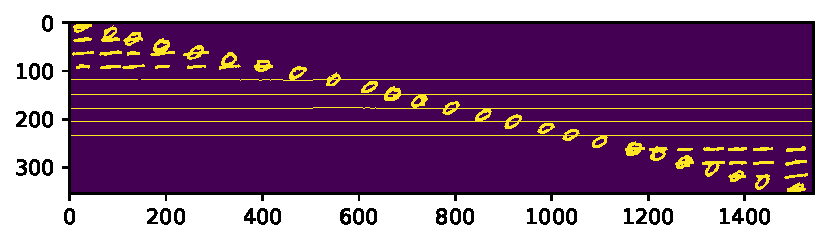
\includegraphics[width=140mm]{../img/test_1}
\caption{Whole notes, descending.}
\label{fig:WholeNotesDescending}
\end{figure}

It is difficult to evaluate an~OMR~system in general. This is because there is no standard dataset that can be used and no standard set of metrics. Moreover, we proposed a~new Mashcima representation for the music engraved in a~staff. This representation is based on the~agnostic encoding proposed by Calvo-Zaragoza and Rizo (\cite{Primus}). Using custom representation makes it yet more difficult to compare our results to other works. That being said, we can still make some comparisons. It seems that having a~specialized engraving system is a~step in the right direction. The results we obtained when evaluating are comparable to similar works performing similar evaluation (\cite{HmrBaseline}).

The~thesis assignment states that the~output of our model will be a~MusicXML file. We quickly realized that the~problem is far larger than anticipated and so we focused on the~core features only. Similarly, the~model input is not a~plain photo or scan. It is already preprocessed and binarized. This problem has already been solved during the~creation of the~CVC-MUSCIMA dataset (\cite{CvcMuscima}), therefore we didn't tackle it either.

Also, there's a~Github repository containing all the~source code and text of this thesis at \href{https://github.com/Jirka-Mayer/BachelorThesis}{\texttt{https://github.com/Jirka-Mayer/BachelorThesis}}. There's also a~release tag corresponding to the~time this thesis was submitted and it contains all the~trained models for download.

\section*{Thesis outline}
\addcontentsline{toc}{section}{Thesis outline}

\paragraph{Chapter 1:} This chapter describes the specific model we decide to use for our OMR task. It discusses traditional methods and how deep neural networks help us simplify the process. It describes models other people used for similar tasks and how we've been influenced by them.

\paragraph{Chapter 2:} This chapter mainly describes the Mashcima music encoding - the encoding we used for our model. It describes how it relates to the PrIMuS agnostic encoding, and why we made certain decisions regarding its design.

\paragraph{Chapter 3:} This chapter talks about the Mashcima engraving system. Why we developed this system and what problem it solves. How it works, what are its limitations, and how it can be extended.

\paragraph{Chapter 4:} This chapter describes the experiments we performed. These experiments aim to measure the performance of our approach and test hypotheses postulated in previous chapters. We will also attempt to compare our results to other similar works.

\chapter*{Related Work}
\addcontentsline{toc}{chapter}{Related work}
\label{chap:RelatedWork}


\section*{CVC-MUSCIMA dataset}
\addcontentsline{toc}{section}{CVC-MUSCIMA dataset}

CVC-MUSCIMA is a~dataset presented in the article: \emph{CVC-MUSCIMA: A ground truth of handwritten music score images for writer identification and staff removal} (\cite{CvcMuscima}). This dataset contains 1000~sheets of~music, consisting of 20~pages, each written by 50~different musicians. It's the~only publicly available dataset containing entire staves of handwritten music. The~dataset has been designed for writer identification and staff (staff line) removal tasks. It contains two sets of images. One set for writer identification (containing gray, binary, and staff-less binary images) and one set for staff removal (contains raw, staff-less, and staff-only images, all binary).

We will use part of the~staff removal set for evaluation. We will also use another part of the~staff removal set for engraving, but indirectly via the MUSCIMA++ dataset.


\section*{MUSCIMA++ dataset}
\addcontentsline{toc}{section}{MUSCIMA++ dataset}

MUSCIMA++ is a~dataset developed by Jan Hajič~jr. and Pavel Pecina and has been presented in the~article: \emph{In Search of a Dataset for Handwritten Optical Music Recognition: Introducing MUSCIMA++} (\cite{MuscimaPP}). This dataset provides additional information for a~subset of the~CVC-MUSCIMA dataset. MUSCIMA++ contains 140~sheets of music. Each sheet is annotated at the~level of individual symbols (noteheads, stems, flags, beams, slurs, staff lines). Each one of these symbols is classified, contains a~bounding box and a~pixel mask. These symbols are then interlinked in a~graph that can be traversed to extract higher-level objects (notes, key signatures, beamed note groups).

We will use the~dataset as a~collection of musical symbols. We will then place those symbols onto an~empty staff to create synthetic training data. The additional data (relationship graph) will help us position certain symbols properly.


\section*{End-to-End OMR and the PrIMuS dataset}
\addcontentsline{toc}{section}{End-to-End OMR and the PrIMuS dataset}

This section refers to the~article: \emph{End-to-End Neural Optical Music Recognition of Monophonic Scores} (\cite{Primus}). This article first describes the~PrIMuS\footnote{\href{https://grfia.dlsi.ua.es/primus/}{https://grfia.dlsi.ua.es/primus/}} dataset. This dataset contains 87678~real-music incipits. An~incipit is the~part of a~melody or a~musical work that is most recognizable for that work. Each incipit is a~few measures long, typically shorter than a~single staff of printed sheet music. Each incipit is encoded in a~few widely known encodings (MEI, MIDI) and has a corresponding printed image. This image has been engraved using the~music notation engraving library Verovio\footnote{\href{https://www.verovio.org/}{https://www.verovio.org/}}. Each incipit is also encoded using two on-purpose devised encodings --- the PrIMuS semantic and agnostic encoding. These encodings are interesting because they are the~output of a~model proposed in the~article, but also the~Mashcima encoding described in chapter \ref{chap:MusicRepresentation} of this thesis is very similar to the~agnostic encoding.

The~article also proposes a~neural network architecture for an~end-to-end solution of~OMR. The~architecture is very similar to ours, almost identical. It also uses the~connectionist temporal classification as the loss function (\cite{CTC}), which shapes the~PrIMuS dataset encoding formats. This thesis differs from this article mainly in the~focus on~handwritten music and the~introduction of~a~custom engraving system for handwritten music. The PrIMuS article focuses on~printed music only.

We will use the~PrIMuS dataset as a~source of~melodies that can be used as~input to~our engraving system. We will also take this article as~a~basis for our Mashcima encoding and our model architecture.


\section*{HMR baseline article}
\addcontentsline{toc}{section}{HMR baseline article}

This section refers to the~article: \emph{From Optical Music Recognition to Handwritten Music Recognition: A baseline} (\cite{HmrBaseline}). This paper proposes a~model that should serve as a~baseline for handwritten music recognition. The model is again a~convolutional recurrent neural network that recognizes entire staves. The model is trained on~printed music and then, using transfer learning, fine-tuned on handwritten music. The handwritten music comes from the~MUSCIMA++ dataset and it has been varied using data augmentation (blurring, erosion, dilation, measure shuffling). This model, however, does not use the CTC loss function, instead, it produces two vectors for each pixel of the~input image width. One vector contains symbols that are present in the~image at~that position and the~other vector contains pitches of~these symbols. This means annotations have to be aligned with the symbols (unlike with CTC), but it allows the~model to recognize dense music sheets and even chords.

We will attempt to compare our model to the~one from this article. The~comparison will be difficult because the~output formats are so~different, but we will mention all the~differences and add a~qualitative comparison of the~final predictions. We want to utilize the fact that our evaluation dataset intersects with theirs and~so we can perform a~direct comparison.

\chapter{Deep Neural Network}
\label{chap:DeepNeuralNetwork}

This chapter talks mainly about the~model we decided to use. First, we describe the~full pipeline of a~traditional OMR system. Many of these steps are shared between traditional and deep learning approaches. Then we will talk about the~deep learning approaches that can be taken. Neural networks can replace parts of a~traditional pipeline, or they can be used in an~end-to-end setting, where the~neural network replaces the~most difficult core of the~pipeline. We will describe our architecture consisting of a~convolutional block, recurrent block, and the~connectionist temporal classification (CTC) loss function. The~following sections describe in more detail what a~neural network is and how the~individual blocks of our model work internally. The~last section explains how CTC works and what are its pros and cons, compared to the~approach described in the~HMR baseline article (\cite{HmrBaseline}).


\section{Traditional approaches}

A~musical score intended for OMR typically begins as a~raster image. This image is a~photo or a~scan of a~real-world sheet of paper. The~image needs to be prepared first. We need to find the~sheet of paper in the~image and correct any rotation or~perspective distortion. Scanned images are easier to~prepare because they don't contain any perspective deformation and lighting artifacts. Searching for the~paper in the~image can be performed using many approaches, e.g. by using maximally stable extremal regions (\cite{MSER}). We can detect staff lines using Hough transform (\cite{Hough}). We can then use this information to remove any affine distortion of the~image.

The~next step is performing some color normalization and binarization. There might be a~light-intensity gradient over the~image, so we do some automatic contrasting to bring the~lightness to a~constant level across the~image. Median filtering can be applied to remove noise (\cite{MedianFiltering}). Conversion to a~grayscale image is often used since colors are not useful to OMR. The~image can then be binarized to further remove unnecessary information. Many thresholding algorithms can be used for this step, many of which are implemented in the~OpenCV\footnote{\href{https://opencv.org/}{https://opencv.org/}} library. Binarization is important for traditional approaches since they often use methods based on connected components to detect individual symbols. Neural networks could benefit from non-binarized images since binarization can create aliasing artifacts that distort the~input image on the~pixel level.

The~steps described above are shared by both traditional and neural network-based approaches. Traditional approaches now usually perform staff line removal. This step lets methods based on~connected components to become useful. Staff localization may be an~important part of this step. Symbols then need to be segmented and classified separately. Meaning is then reconstructed by looking at the~relationships between all the~classified symbols. With the~musical score understood at the~symbol level, the~extracted information can be converted to some final representation (MusicXML, MEI, MIDI).


\section{Deep learning approaches}

Deep learning is a~class of machine learning that focuses on deep neural networks. Deep learning has risen over the~past two decades and became a~very powerful tool for solving many problems, especially classification problems regarding computer vision. Neural networks can be used in many places throughout the~pipeline of a~traditional OMR system. They can be used for staff line removal (\cite{CalvoZaragoza2017}), symbol classification (\cite{Lee2016}), or even symbol detection (\cite{Pacha2018}).

Recently, neural networks have been used to tackle the~problem of~OMR in an~end-to-end fashion (\cite{Primus}, \cite{HmrBaseline}). This approach allows us to replace many stages of the~pipeline with a~single model. The input sheet of music is usually processed staff by staff, so an~initial segmentation of staves is required. This step is, however, very robust and can be performed reliably.

The~main steps unified by an~end-to-end system are segmentation, symbol classification, and part of the~relationship extraction. This means we don't need to explicitly specify the~structure of this part of the~pipeline, which saves a~lot of time and thinking. Also, any intermediate features that would be extracted (like noteheads) need not be specified. The deep neural network can learn, what those features are. Moreover, it can adapt these features to the problem better than a~human could.

Deep learning, especially in an~end-to-end approach also has some drawbacks. The first is bound to the ability of the~model to learn the~solution from data. While it's very helpful, that we don't have to design part of our OMR system manually, it's often very difficult to acquire enough high-quality data for the~training. Also, the~more complex our model is and the~more learned parameters it has, the~more training data it requires. The~data also needs to be of high quality. Ambiguity and mistakes in annotations lead to poor performance of the~resulting model. The~trained model can only ever be as good as it's training data.

The second drawback is the~very difficult nature of debugging the~model. A neural network is by design a~black box and we cannot easily assign specific meaning to any of its internal parts. The process of fixing a~mistake the model makes is tedious and requires a~lot of experimentation and re-training.


\section{Our architecture}

As stated in the~title of this thesis, we decided to explore the~end-to-end approach to OMR using deep neural networks. We were primarily inspired by these three models:

\begin{itemize}
\item End-to-End Neural Optical Music Recognition of Monophonic Scores by Calvo-Zaragoza and Rizo (\cite{Primus})
\item SimpleHTR by Harald Scheidl\footnote{\href{https://github.com/githubharald/SimpleHTR}{https://github.com/githubharald/SimpleHTR}}
\item From Optical Music Recognition to Handwritten Music Recognition: A baseline (\cite{HmrBaseline})
\end{itemize}

All of these models share the~same high-level structure. They combine a~convolutional neural network (CNN) with a~recurrent neural network (RNN). This combination is sometimes called RCNN architecture. Convolutional neural networks are used in image processing. Their architecture is inspired by the~way filters work in computer graphics (convolving a~kernel over the~source image). They learn to extract edges, corners, and then even more abstract features like noteheads and stems. Recurrent neural networks are used for sequence processing (text and speech). They have been designed to carry state information throughout the~input sequence. In our case, they learn to propagate information horizontally - like inferring pitch of an~accidental from the~pitch of a~neighboring note. The CNN block learns to extract features that the RNN block then learns to combine into more abstract features.

\begin{code}
image of the blocks
(image -> cnn -> rnn -> ctc -> resulting vectors)
\end{code}

The~CNN block can be followed by fully connected layers that further refine the~result, although these layers are not necessary and our architecture doesn't contain them. This may be due to the fact that our encoding is very close to the~symbolic visual representation and~so most of the~heavy lifting is probably performed in the~CNN block.

The~final layer outputs a~sequence of vectors, where each vector represents one time-step (horizontal slice of the~input image). Values in such vector correspond to probabilities of individual output classes (tokens) at that given time-step. One additional class \emph{blank} is added, which represents "no symbol present". The~most likely class for each time-step is selected and then repetitions of the~same class are collapsed into one token. Lastly, all the~blank symbols are removed. The~remaining sequence of classes is mapped directly onto annotation tokens of the~Mashcima encoding explained in the~chapter \ref{chap:MusicRepresentation}. This approach is called greedy CTC decoding (\cite{CTC}) and is used during training. For evaluation, a more advanced method is used, called beam search decoding (\cite{CtcBeamSearch}).

When training, the~loss is computed using the~connectionist temporal classification. The~loss function provides a~gradient for improving the~network. This gradient is then calculated for the~entire network using the~backpropagation algorithm (\cite{Goodfellow-et-al-2016}). Parameters are then updated using the~adaptive learning rate optimizer (Adam) (\cite{AdamOptimizer}).

The~values of all hyperparameters, including sizes and types of all layers, are specified in the~section \ref{sec:ArchitectureTrainingEvaluation}.


\subsection{Neural network}


\subsection{Convolutional neural network}


\subsection{Recurrent neural network}


\subsection{Connectionist temporal classification}

\chapter{Title of the second chapter}

\section{Title of the first subchapter of the second chapter}

\section{Title of the second subchapter of the second chapter}

\chapter{Engraving system}
\label{ChapterEngravingSystem}

\section{Title of the first subchapter of the third chapter}

\section{Title of the third subchapter of the second chapter}

\chapter{Experiments and Results}
\label{chap:ExperimentsAndResults}

\section{Title of the first subchapter of the fourth chapter}

\section{Title of the fourth subchapter of the second chapter}


\chapter*{Conclusion}
\addcontentsline{toc}{chapter}{Conclusion}


%%% Bibliography
%%% Bibliography (literature used as a source)
%%%
%%% We employ bibTeX to construct the bibliography. It processes
%%% citations in the text (e.g., the \cite{...} macro) and looks up
%%% relevant entries in the bibliography.bib file.
%%%
%%% The \bibliographystyle command selects, which style will be used
%%% for references from the text. The argument in curly brackets is
%%% the name of the corresponding style file (*.bst). Both styles
%%% mentioned in this template are included in LaTeX distributions.

\bibliographystyle{plainnat}    %% Author (year)
% \bibliographystyle{unsrt}     %% [number]

\renewcommand{\bibname}{Bibliography}

%%% Generate the bibliography. Beware that if you cited no works,
%%% the empty list will be omitted completely.

\bibliography{bibliography}

%%% If case you prefer to write the bibliography manually (without bibTeX),
%%% you can use the following. Please follow the ISO 690 standard and
%%% citation conventions of your field of research.

% \begin{thebibliography}{99}
%
% \bibitem{lamport94}
%   {\sc Lamport,} Leslie.
%   \emph{\LaTeX: A Document Preparation System}.
%   2nd edition.
%   Massachusetts: Addison Wesley, 1994.
%   ISBN 0-201-52983-1.
%
% \end{thebibliography}


%%% Figures used in the thesis (consider if this is needed)
\listoffigures

%%% Tables used in the thesis (consider if this is needed)
%%% In mathematical theses, it could be better to move the list of tables to the beginning of the thesis.
\listoftables
\XXX{In mathematical theses, it could be better to move the list of tables to the beginning of the thesis.}

%%% Abbreviations used in the thesis, if any, including their explanation
%%% In mathematical theses, it could be better to move the list of abbreviations to the beginning of the thesis.
\chapwithtoc{List of Abbreviations}
\XXX{In mathematical theses, it could be better to move the list of abbreviations to the beginning of the thesis.}

%% PHDONLY
%%% Doctoral theses must contain a list of author's publications
\chapwithtoc{List of publications}
\XXX{Doctoral theses must contain a list of author's publications.}
%% ONLYPHD

%%% Attachments to the bachelor thesis, if any. Each attachment must be
%%% referred to at least once from the text of the thesis. Attachments
%%% are numbered.
%%%
%%% The printed version should preferably contain attachments, which can be
%%% read (additional tables and charts, supplementary text, examples of
%%% program output, etc.). The electronic version is more suited for attachments
%%% which will likely be used in an electronic form rather than read (program
%%% source code, data files, interactive charts, etc.). Electronic attachments
%%% should be uploaded to SIS and optionally also included in the thesis on a~CD/DVD.
%%% Allowed file formats are specified in provision of the rector no. 72/2017.
\appendix
\chapter{Attachments}
\XXX{Attachments to the bachelor thesis, if any. Each attachment must be referred to at least once from the text of the thesis. Attachments are numbered.}
\XXX{The printed version should preferably contain attachments, which can be read (additional tables and charts, supplementary text, examples of program output, etc.). The electronic version is more suited for attachments which will likely be used in an electronic form rather than read (program source code, data files, interactive charts, etc.). Electronic attachments should be uploaded to SIS and optionally also included in the thesis on a~CD/DVD. Allowed file formats are specified in provision of the rector no. 72/2017.}

\section{First Attachment}

\openright
\end{document}
